The \href{{https://github.com/tue-robotics/ed_localization}}{\acrshort{ed}-localization plugin} implements \acrshort{amcl} based on a 2D render from its world model.

%In order to navigate, a model of the environment is required. This model is stored in the (\acrshort{ed}). From this model, a planning representation is derived that enables using the model of the environment for navigation purposes.
%\begin{figure}[hb]
%    %\vspace{-0.3cm}
%	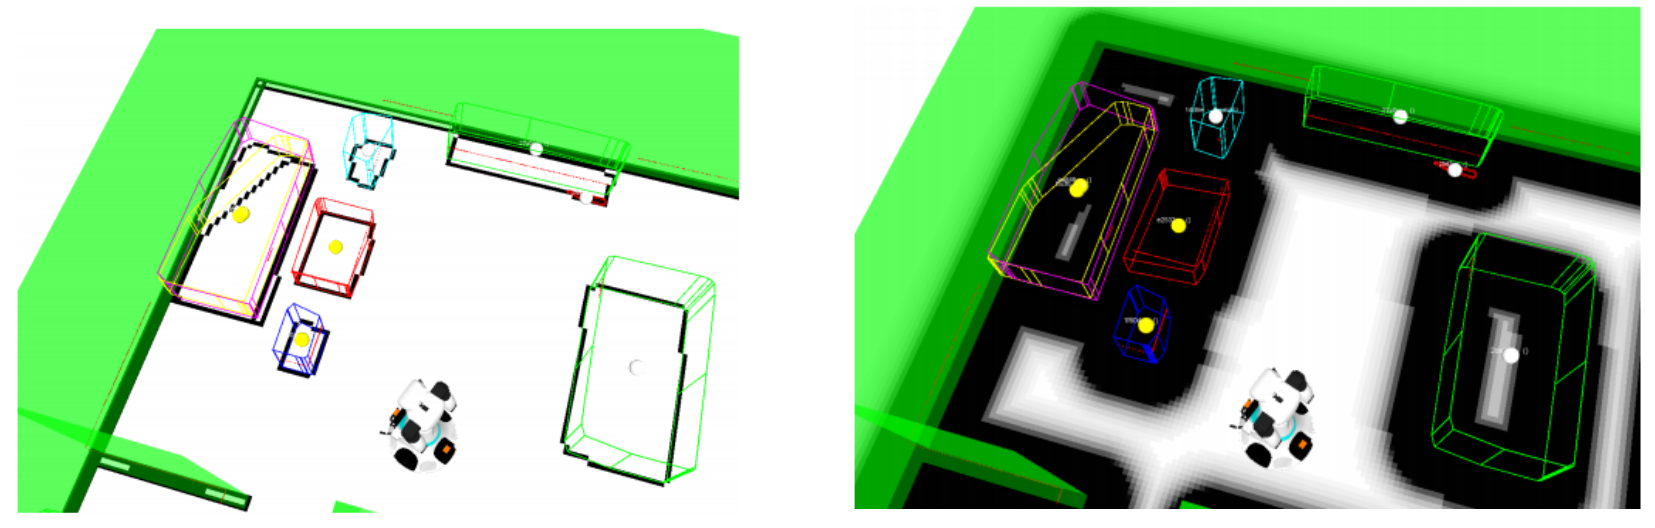
\includegraphics[width = \linewidth]{Figures/ed_navigation}
%    %\vspace{-1em}
%	\caption{Grid representation of the environment.}
%	\label{fig:ed_navigation}
%    %\vspace{-0.2cm}
%\end{figure}
With use of the \href{https://github.com/tue-robotics/ed_navigation}{ed\_navigation plugin}, an occupancy grid is derived from the world model and published as a nav\_msgs/OccupancyGrid. This grid can be used by a motion planner to perform searches in the configuration space of the robot.
\\
With the use of the \href{https://github.com/tue-robotics/cb_base_navigation}{cb\_base\_navigation} ROS package. The robots are able to deal with end goal constraints. With use of a ROS service, provided by the ed\_navigation plugin, an end goal constraint can be constructed w.r.t. a specific world model entity described by ED. This enables the robot to not only navigate to poses but also to areas or entities in the scene, as illustrated by Figure \ref{fig:ed_navigation_constraints}.
\begin{figure}[h]
    \centering
    %\vspace{-0.2cm}
	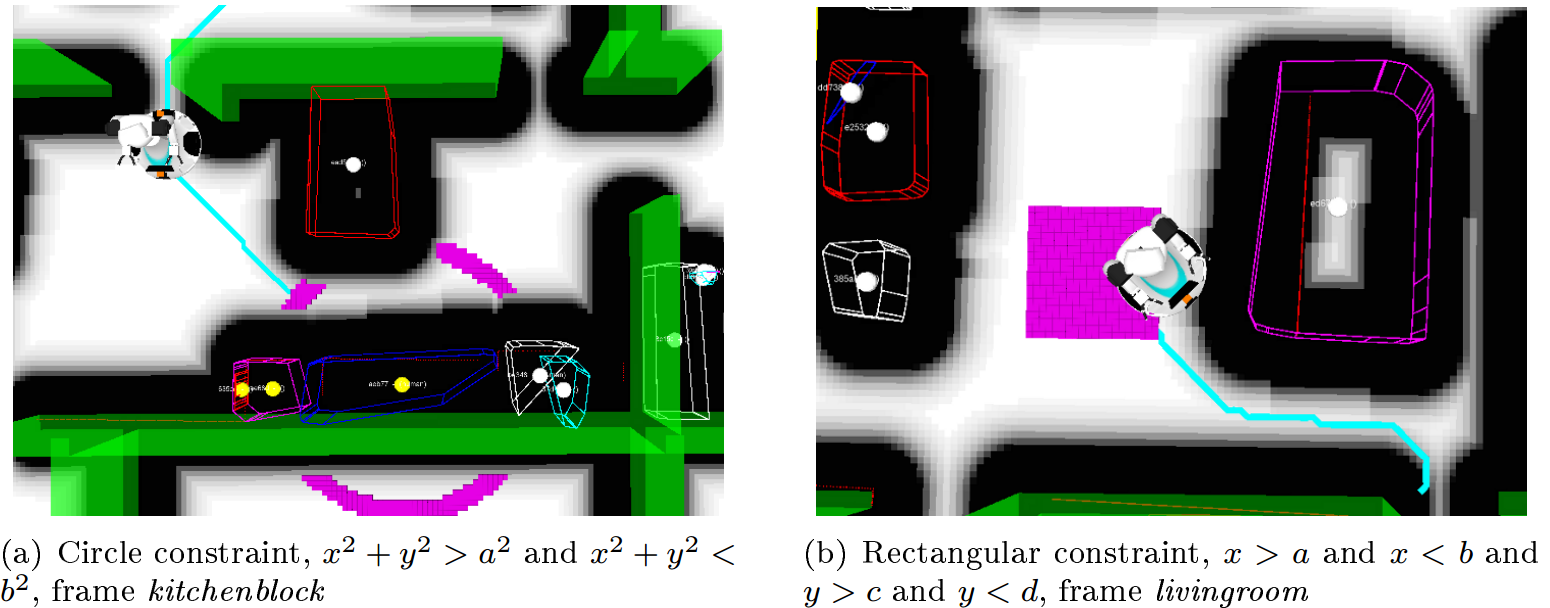
\includegraphics[width = 0.9\linewidth]{Figures/ed_navigation_constraints}
    %\vspace{-0.5em}
	\caption{Navigation position constraints w.r.t. other entities in the environment}
	\label{fig:ed_navigation_constraints}
    %\vspace{-0.5cm}
\end{figure}
Somewhat modified versions of the local and global ROS planners available within move\_base are used. \\The configurations for move\_base node has now been created for the AMIGO and SERGIO robots, the HSR node will be added. The node integrates local and global path planning and local control. Its actionlib interface has become in fact standard for sending 2D navigation goals to robots in ROS. 